\documentclass[11pt,conference,draftcls,onecolumn]{IEEEtran}
\pagestyle{plain}
\IEEEoverridecommandlockouts
% The preceding line is only needed to identify funding in the first footnote. If that is unneeded, please comment it out.
\usepackage{cite}
\usepackage{amsmath,amssymb,amsfonts}
\usepackage{algorithmic}
\usepackage{graphicx}
\usepackage{textcomp}
\usepackage{xcolor}
\def\BibTeX{{\rm B\kern-.05em{\sc i\kern-.025em b}\kern-.08em
    T\kern-.1667em\lower.7ex\hbox{E}\kern-.125emX}}
\begin{document}

\title{Online Anomaly Detection in Request-Based Battery Management Systems\\
{}
\thanks{This work was funded in part by NSF Grant No. 1234567}
}

\author{\IEEEauthorblockN{Aaron Willcock}
\IEEEauthorblockA{\textit{Department of Computer Science} \\
\textit{Wayne State University}\\
Detroit, MI, USA \\
aaron.willcock@wayne.edu}
\and
\IEEEauthorblockN{Nathan Fisher}
\IEEEauthorblockA{\textit{Department of Computer Science} \\
\textit{Wayne State University}\\
Detroit, MI, USA \\
fishern@wayne.edu}
}

\maketitle

\begin{abstract}
Battery Management System (BMS) research has included reconfigurable cell architecture, state of health estimation, battery balancing, and real-time scheduling.
However, anomaly detection in BMSs is addressed only as an offline method for identifying malfunctions or parasitic loads.
Furthermore, the costly implementation of BMSs has resulted in few works evaluating approaches outside of simulation.
In this report, a low-cost BMS is designed and implemented with an online anomaly detection system to mitigate damage in real-time.   
\end{abstract}

\begin{IEEEkeywords}
battery management system, anomaly detection, real-time systems
\end{IEEEkeywords}

\section{Introduction}
The number of plug-in electric vehicles (hybrid and pure-electric) is expected to reach over 70 million by 2030 according to the International Energy Agency \cite{iea}.
Electric vehicles typically contain a Battery Management System (BMS) responsible for handling the charging, discharging, reconfiguration, monitoring and control of the vehicles batteries.
Recent BMS research has included architecture of reconfigurable cells, state of health estimation, battery balancing, and real-time scheduling
\cite{batteryAwareDynamicSchedulingForPeriodicTaskGraphs,realTimePredictionOfBatteryPowerRequirements,reconfigurableBatteryTechniquesAndSystems}.
However, BMSs are expensive to purchase and as a result many research projects concerning BMS architecture (both physical and digital) are evaluated in simulation only \cite{towardsSmarterBatteryDesign}.
To the best of our knowledge, few works have implemented a low-cost BMS system and no works have addressed online anomaly detection in the operation and communication of BMSs.
Furthermore, we are not aware of any works which govern BMS supply on a request basis.

As such, we view the lack of online anomaly detection in BMS operation and communication as an opportunity to design fault-detection behavior for load-aware BMS.
The absence of request-based in existing BMS architectures is another opportunity for applying real-time systems concepts to anomaly detection.
Finally, this project tangentially addresses the challenge of producing a low-cost physical realization to help make BMS implementation and testing more accessible by lowering the cost of entry.

\subsection{Research Questions and Project Goal}
Formally, our research questions are as follows:
\begin{enumerate}
    \item What anomalies can exist in a BMS?
    \item How can request-based communication between a load manager and BMS be used to implement and/or improve anomaly detection?
    \item What design would facilitate a low-cost implementation and evaluation of online anomaly detection in a request-based BMS?
\end{enumerate}

The overarching goal of this project is to create a joint Load Management System (LMS) and BMS that is: low cost in manufacturing and materials cost;
allows for the creation, acceptance, rejection, and enforcement of load schedules;
and detects system anomalies including over-voltage, under-voltage, over-current, under-current, and load mismatch.

\subsection{Contributions}
The contributions of this project report are summarized as:
\begin{enumerate}
    \item a low-cst BMS-LMS model,
    \item a protocol for request-based BMS-LMS communication,
    \item a set of online anomaly detection methods based on the above model and protocol, and
    \item a low-cost BMS-LMS system implmentation that demonstrates anomaly detection.
\end{enumerate}

\subsection{Report Outline}
The remainder of the report is as follows.
Section \ref{sec:relatedWork}, Related Work, covers related work in topics including batteries, battery management systems, and real-time systems.
Section \ref{sec:systemModel}, System Model, defines the system model including the Battery Management and Load Management Systems.
Section \ref{sec:rbComm}, Request-Based Communication, explains the request-based communication protocol.
Section \ref{sec:anomalyDetection}, Anomaly Detection, discusses the types of anomalies that may occur in BMSs and the approaches taken to detect them in this project.
Section \ref{sec:experiments}, Experiments, lists the experimental setup, execution, and experiments themselves to evaluate the efficacy of the online anomaly detection approach.
Section \ref{sec:results}, Results, describes the results of the aforementioned experiments.
Section \ref{sec:discussion}, Discussion, identifies weaknesses in the model and approach, implementation challenges, and deferred objectives.
Section \ref{sec:conclusion}, Conclusion, concludes the report with a summary of contributions and future work. 

\section{Related Work}\label{sec:relatedWork}
The state-of-the-art in battery management systems as it pertains to real-time systems focuses on two topics: batteries (and the BMSs that manage them) and real-time, cyber-physical systems.
Work that focus on batteries or BMSs exclusively tend to be hardware-oriented while cyber-physical and real-time systems works are either a blend of hardware and algorithms or algorithms exclusively.
The following subsections highlight some relevant works in these topics.

\subsection{Batteries and Battery Management Systems}
Relevant battery-specific research includes recent works on software-defined batteries \cite{softwareDefinedBatteriesConf,softwareDefinedBatteriesJrnl}.
In software-defined batteries, batteries of different chemistries may be combined to leverage the benefits of both chemistries.
Through fast switching, batterying charging and discharging can be optimized by distributing the energy load according to battery type.

In a less-flexible sense, other batteries leverage software to closely monitor individual cells and provide load balancing across those cells with the goal of extending battery lifetime \cite{towardsSmarterBatteryDesign}.

Other works address the design of switches around batteries to maximize reconfigurability of batteries while minimizing hardware cost \cite{reconfigurableBatteryTechniquesAndSystems}.
In reconfigurable batteries, cells may rearrange the order in which electrons pass through them (ex. series vs parallel) to change maximum current and voltage delivery online.
Reconfigurable batteries also allow the BMS to completely remove cells which are reducing the performance of neighboring cells \cite{aCaseStudyOnImprovingCapacityDeliveryOfBatteryPacksViaReconfiguration}.

\subsection{Real-Time and Cyber-Physical Systems}
From the cyber-physical and real-time systems perspective, research on BMSs may be aware of electro-chemical properties and hardware cost but focuses more on exploitable properties of the hardware, computational cost, and scheduling.

In the most inflexible case of battery management systems, Liang He provided an approach for state of health estimation in mobile devices which lack coulomb counters \cite{batterySoHEstimationMobile}.
Other works address real-time prediction of power requirements for hybrid and electric vehicles \cite{realTimePredictionOfBatteryPowerRequirements} and online thermal management for BMSs \cite{realTimeBatteryThermalManagement}.

From a pure scheduling standpoint, some works provide scheduling approaches that leverage Dynamic Voltage and Frequency Scaling (DVFS) along with models of constrained power supplies (batteries) to maximize computation while minimizing energy usage (thus extending the amount of computation which may be performed) \cite{batteryAwareDynamicSchedulingForPeriodicTaskGraphs}.

\section{System Model}\label{sec:systemModel}

Motivated by the absence of online anomaly detection for battery management systems, the following section provides an overview of the system model and its two primary components: the BMS and the Load Management System (LMS).

\subsection{System Overview}
The proposed system model contains both a BMS and LMS which act as two nodes in control of the supply and demand of energy respectively.
Figure \ref{fig:bmsModel} depicts a high-level schematic of what devices the BMS and LMS are connected to and responsible for.
The BMS is responsible for monitoring current flow out of the cell.
The LMS is responsible for characterizing the attached system loads and communicating with the BMS over UDP to request permission to active the system loads.
The following subsections will describe implementation-specific points about the BMS and LMS.
\begin{figure}
    \centering
    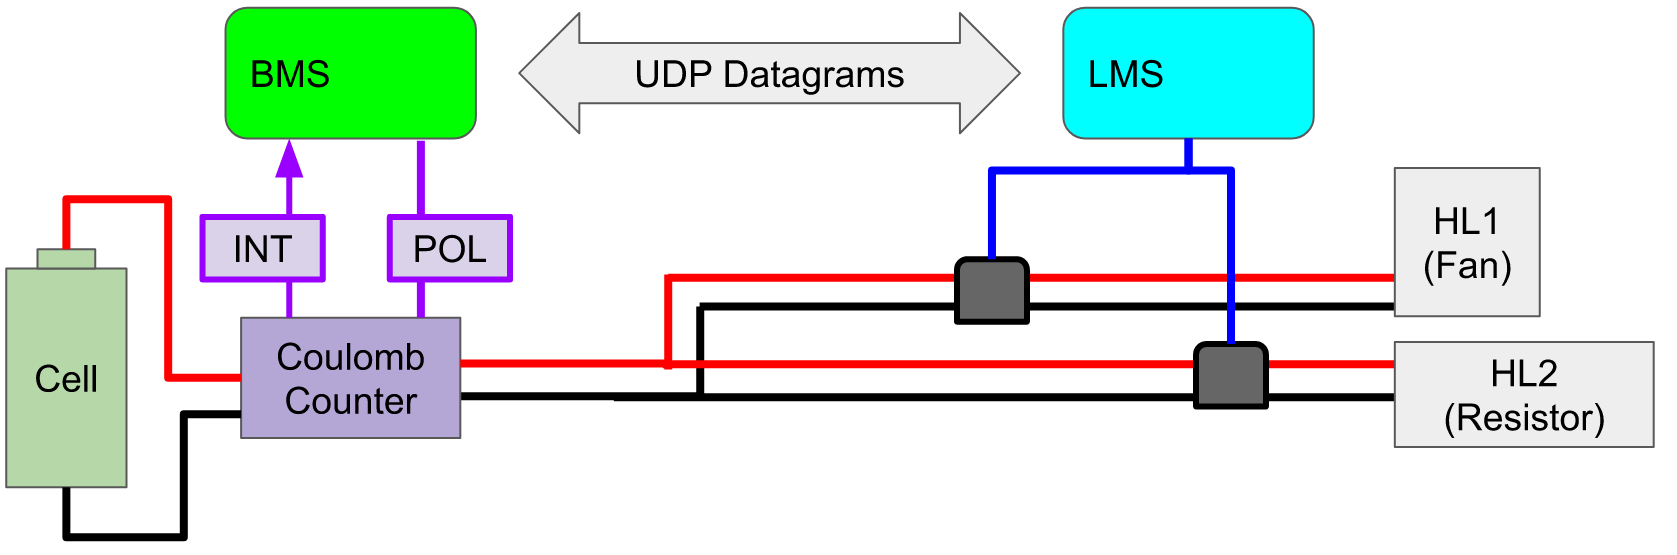
\includegraphics[width=6.5in]{img/uBmsModel.png}
    \caption{BMS and LMS Schematic}
    \label{fig:bmsModel}
\end{figure}

\subsection{Battery Management System Architecture}
In the implementation, the BMS is a Raspberry Pi Zero W \cite{rpiZeroW} which is connected to an LTC4150 Coulomb Counter breakout board.
Figure \ref{fig:coulombCounter} depicts the LTC4150 Coulomb Counter breakout board and its pin names.
The LTC4150 Coulomb Counter breakout board is connected to the nickel–metal hydride (NiMH) battery cells pictured in Figure \ref{fig:nimhBatt}.
Each NiMH cell provides 1.2 V and around 1200mAh of charge.
The NiMH configuration for this project was four cells in series bringing the voltage to 4.8V while maintaining 1200mAh of charge.
This battery model is stored in the BMS for use in accepting and rejecting loads that match the battery configuration - as will be discussed later.

The Raspberry Pi Zero W is configured to fire an interrupt service routine (ISR) on each falling edge of the General Purpose Input-Output (GPIO) port connected to the interrupt port (INT) of the LTC4150 Coulomb Counter (see figure for INT pin).
The LTC4150 Coulomb Counter's INT pin voltage falls low (signaling an interrupt) each time 0.614439C flows through the IN pins and out through the OUT pins - in either direction.
The polarity pin (POL) indicates the in which the 0.614439C has traveled.
By sampling the POL pin each time the ISR is fired, the BMS may track the current flow through (and remaining charge in) the monitored battery. 
\begin{figure}
    \centering
    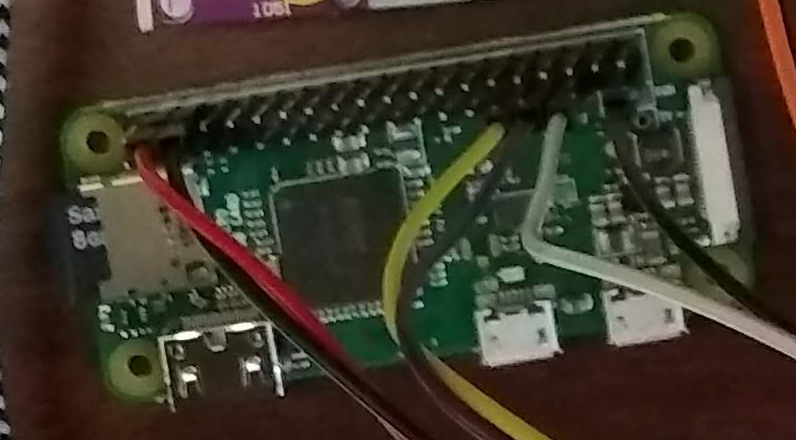
\includegraphics[width=3.5in]{img/rpi0w.png}
    \caption{Raspberry Pi Zero W as a BMS}
    \label{fig:rpi0w}
\end{figure}
\begin{figure}
    \centering
    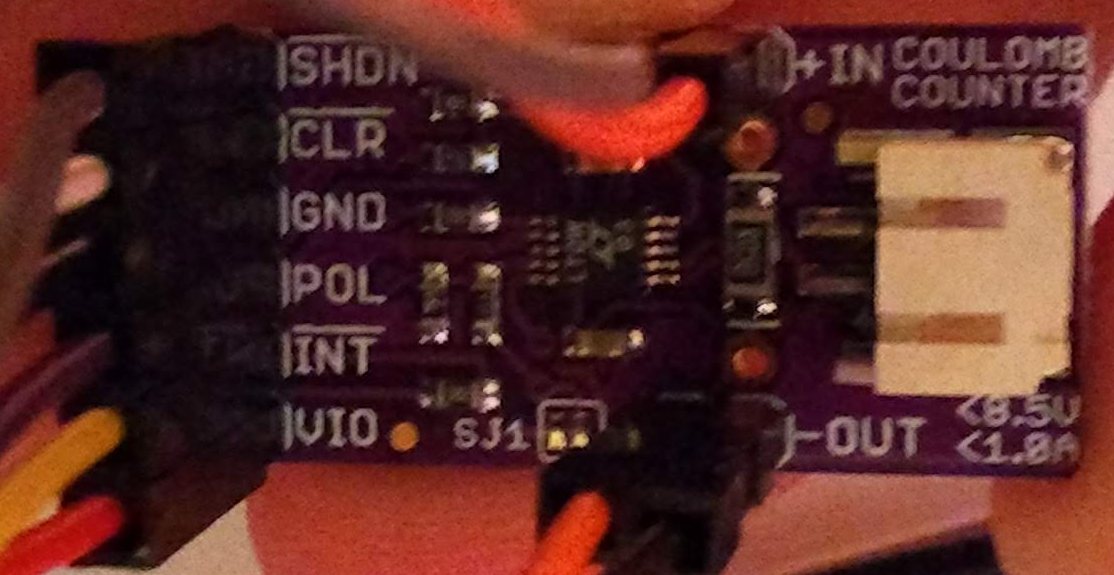
\includegraphics[width=4.5in]{img/coulombCounter.png}
    \caption{An LTC4150 Coulomb Counter Breakout Board}
    \label{fig:coulombCounter}
\end{figure}
\begin{figure}
    \centering
    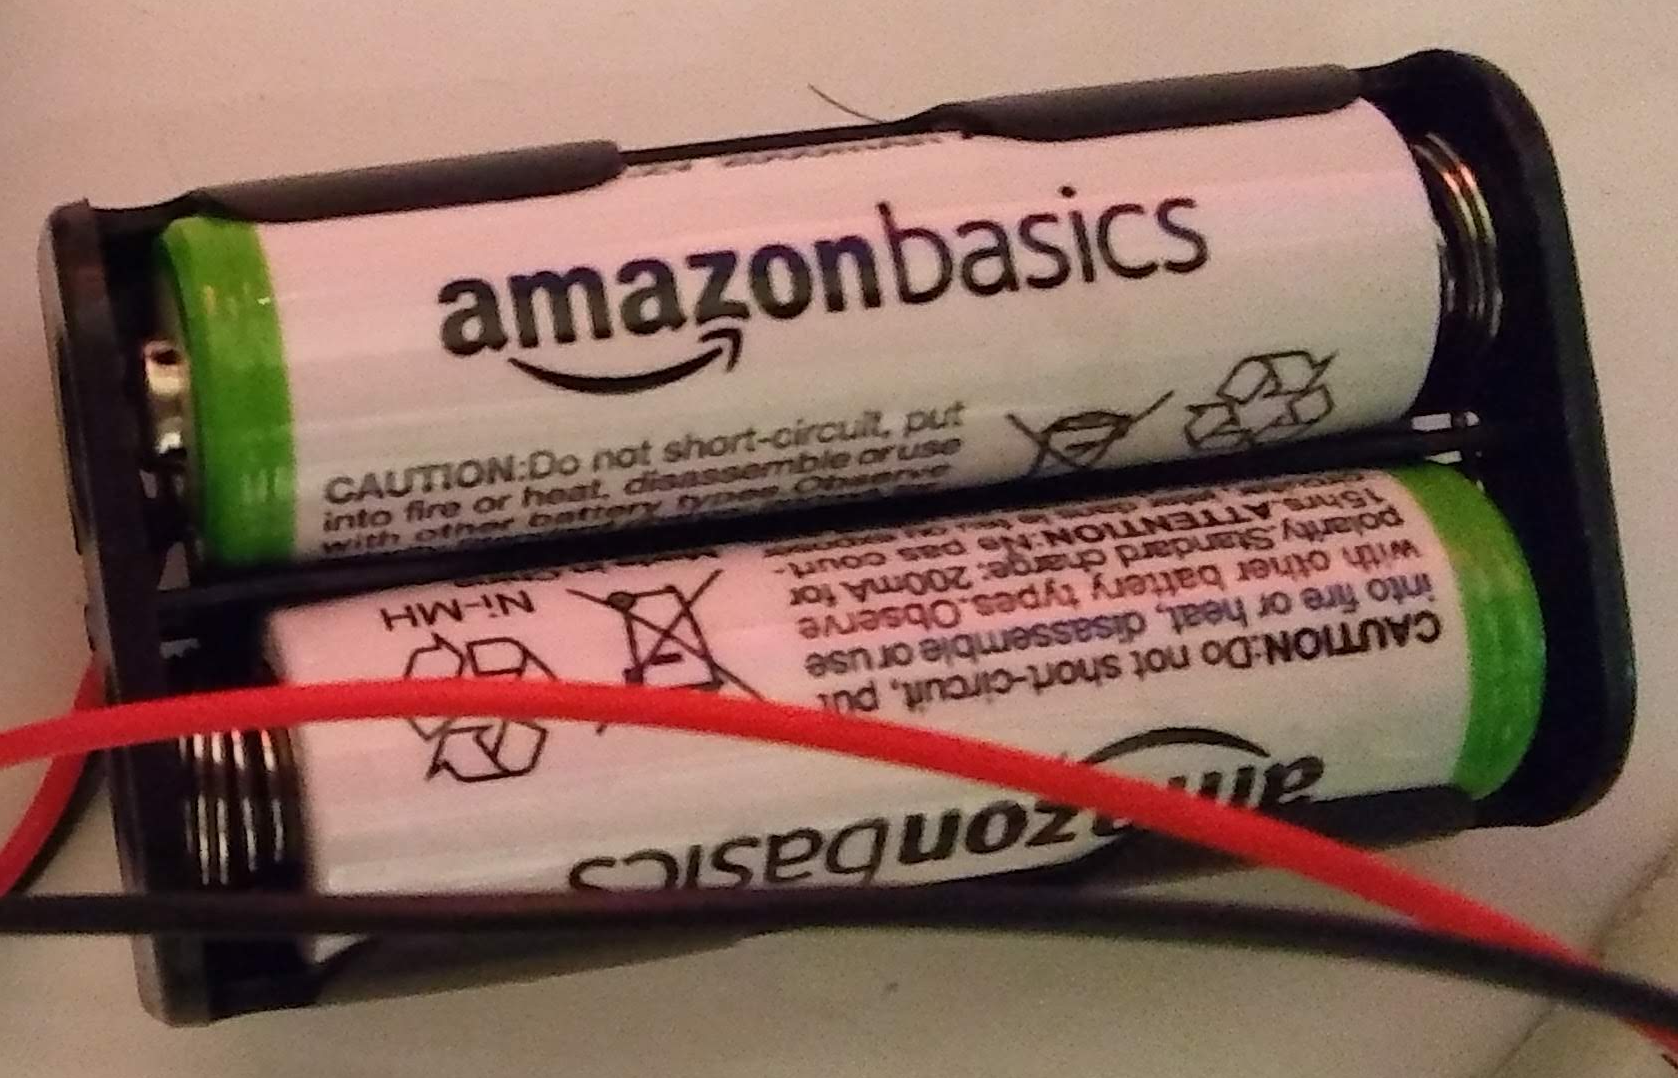
\includegraphics[width=3.5in]{img/nimhBatt.png}
    \caption{1.2V Ni-Mh Batteries}
    \label{fig:nimhBatt}
\end{figure}

\subsection{Load Management System Architecture}
\begin{figure}
    \centering
    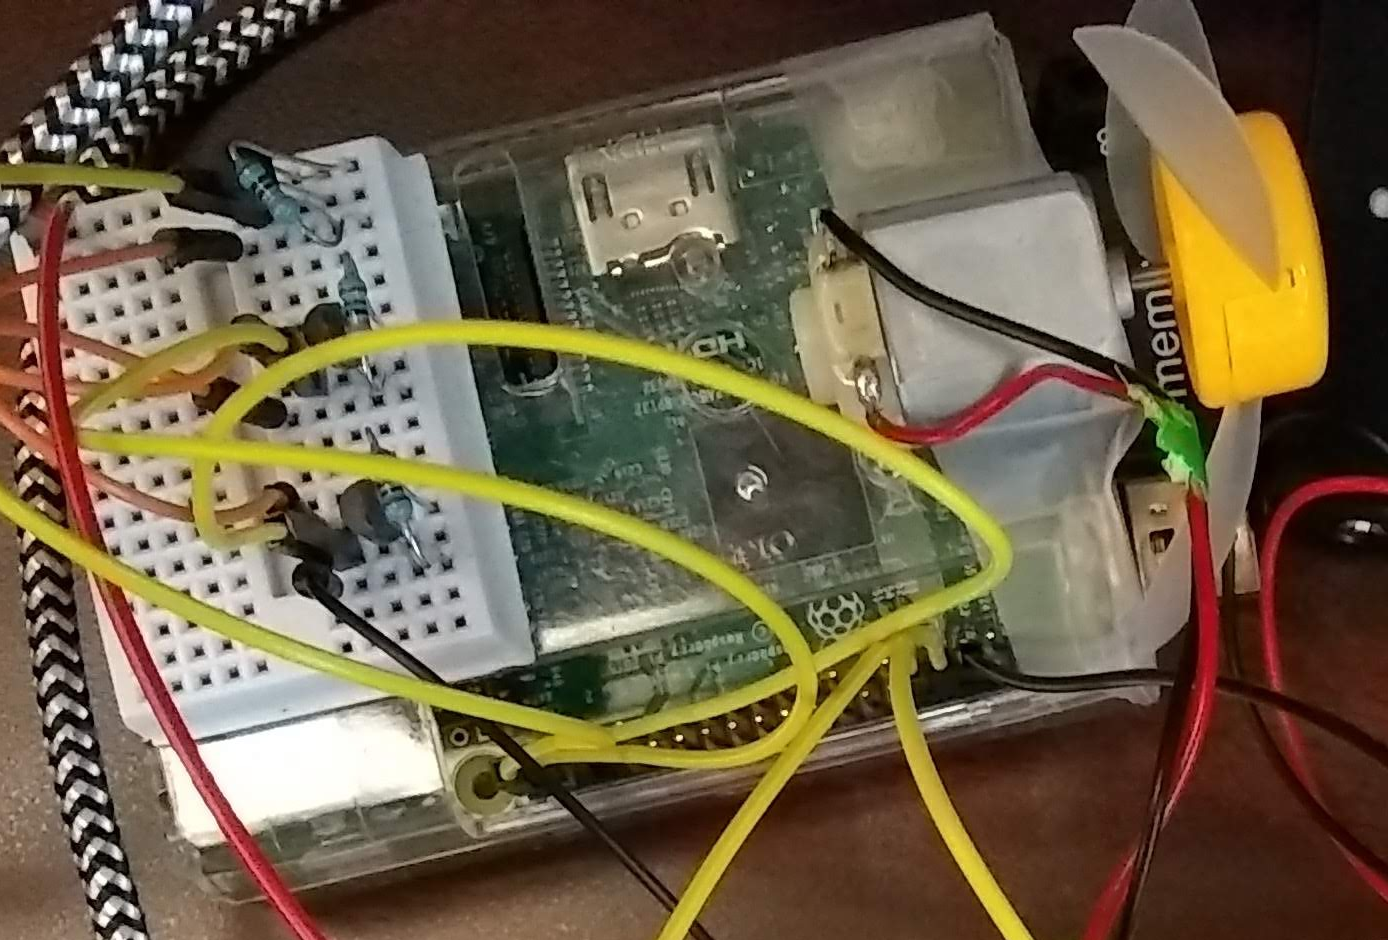
\includegraphics[width=6.5in]{img/rpi3.png}
    \caption{Raspberry Pi 3}
    \label{fig:rpi3}
\end{figure}

\subsection{System Model Summary}

\begin{figure}
    \centering
    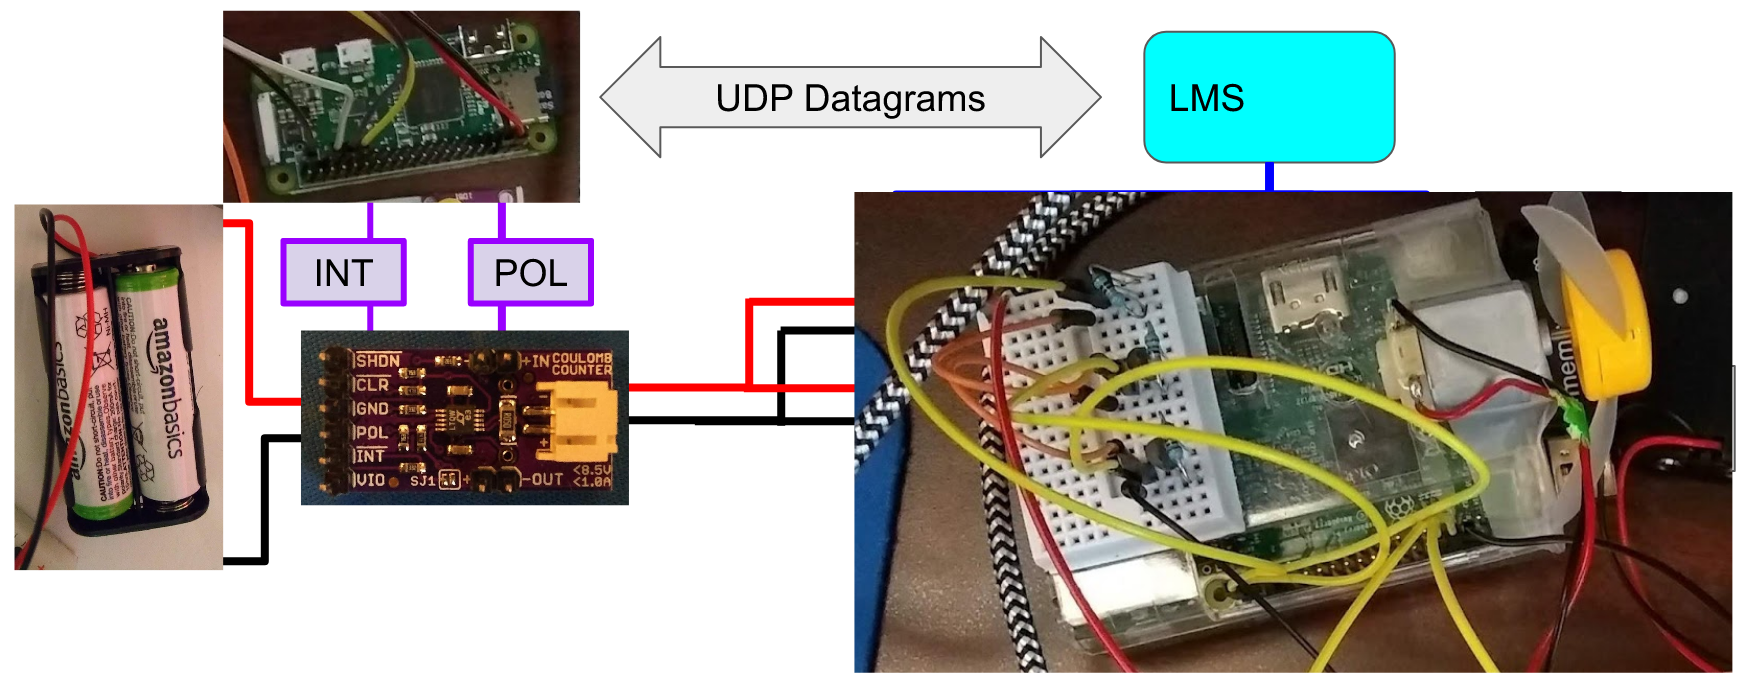
\includegraphics[width=6.5in]{img/uBmsModelPics.png}
    \caption{BMS and LMS Schematic}
    \label{fig:bmsModelPics}
\end{figure}

\section{Request-Based Communication Protocol}\label{sec:rbComm}
\subsection{Load Requests}
\subsection{Load Request Replies}

\section{Anomaly Detection Methods}\label{sec:anomalyDetection}
\subsection{BMS Anomalies}
\subsection{Anomalies Covered}
\subsubsection{Over Voltage}
\subsubsection{Under Voltage}
\subsubsection{Over Current}
\subsubsection{Under Current}
\subsubsection{Load Mismatch}

\section{Experiments}\label{sec:experiments}
\subsection{Experimental Setup}
\subsection{Experimental Execution}
\subsubsection{Over Voltage}
\subsubsection{Under Voltage}
\subsubsection{Over Current}
\subsubsection{Under Current}
\subsubsection{Load Mismatch}

\section{Results}\label{sec:results}
\subsubsection{Over Voltage}
\subsubsection{Under Voltage}
\subsubsection{Over Current}
\subsubsection{Under Current}
\subsubsection{Load Mismatch}

\section{Discussion}\label{sec:discussion}
\subsection{Model Weaknesses}
\subsubsection{Hardware}
\subsubsection{Networking}
\subsubsection{Anomaly Detection}
\subsection{Implementation Challenges}
\subsubsection{Hardware}
\subsubsection{Software}
\subsection{Deferred Objectives}
\subsubsection{Controller Area Network Communication}
\subsubsection{Min/Max Energy Consumption}
\subsubsection{Peak Shaving via Sliding Windows}

\section{Conclusion and Future Work}\label{sec:conclusion}
\section*{Informal Discussion for Professor Fisher}
\subsection{Coulomb Counters as a Limiting Factor}

\bibliography{uBms}
\bibliographystyle{abbrv}

\end{document}
